\subsection{Analysis of the original system} \label{section:improvementsfromoriginal}

\subsubsection{Service description}
The Blocket Secure Package service itself is an additional feature of Blocket.se. As mentioned in Section \ref{section:securepackage}, it is aimed to ensure that the condition of the goods meets the buyer's expectations. The buyer is refunded if the item's conditions are not the same as was specified in the advertisement. Another thing to consider is that, sometimes, parcels tend to get lost by the logistics companies during the transfer. By using Secure Package, the buyer does not have to pay for the item until it is delivered, thus eliminating the risk for paying in advance for something, which ends up getting lost in process of delivery. This service is provided at an additional cost to the seller and the price depends on the size and weight of the item.

\subsubsection{Concept of agreement}
When the buyer and the seller are participating in a transaction, using Blocket Secure Package, they are binding themselves to an agreement between them both, as well as Blocket. This agreement describes the rule-based flow of events, which defines the service and its semantics. The agreement is active from the point when both parties accept the terms for transfer of goods (such as price, condition, etc.) to the point when the item is either accepted by the buyer, or returned to the seller (in case of buyer being unsatisfied with item's condition). The flow of events during the course of the agreement is visualized in form of an action diagram in Figure \ref{fig:agreementaction}.

\begin{figure}[H]
\centering
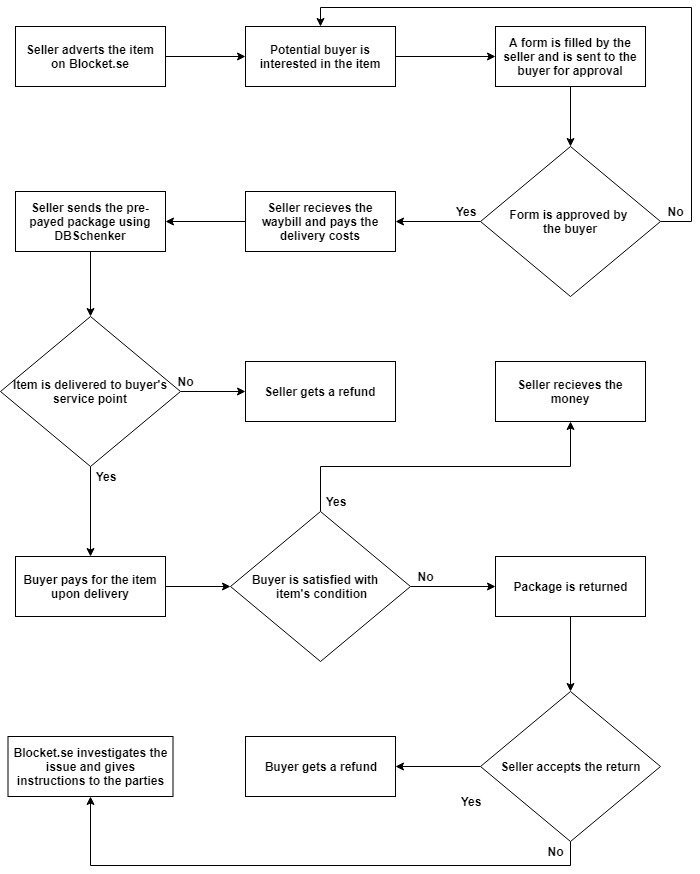
\includegraphics[scale=0.55]{images/actiondiagram.jpg}
\caption{Visualization of the agreement's semantics in form of an action diagram. Some actions are combined for simplification purposes.}
\label{fig:agreementaction}
\end{figure}

Some cases are not included in the action diagram, such as item being lost on the way back to the seller, if it was returned. Actions, like conflict resolving by Blocket were simplified and combined into one action. The reason behind that is to make the diagram more comprehensible and easy to understand.

\subsubsection{Introduction of sensor support} \label{section:additional functionality}
During past years, the Swedish Post (Postnord) suffered from a large increase in lost and damaged packages, due to several reasons, which are not important for this analysis \citep{poststats}. Blocket Secure Package has a partnership with Postnord's competitor, DBSchenker, but the fact that the percentage of lost and damaged packages increases is still relevant. Logistics companies are aware of that and provide a selection of different insurances for packages. This is a good solution for people that send packages, that contain items of great value. However, if the item gets damaged on the way to the destination, the process of proving that the package was damaged during the transfer can become very stressful and frustrating, as the logistics company may try to make the sender prove the fact, that the item was not damaged before it was sent.

An introduction of sensor support would potentially solve that issue. An accelerometer, attached to the package may, for example, be used as a proof that the item was dropped by the logistics company's employee during the transfer. In general, the sensors can be configured with predefined thresholds and have a functionality that would generate an alert once the threshold is violated. The violation of such threshold will act as a proof that the logistics company should be held responsible for damaging the contents of the package, in case of goods being damaged upon delivery. Another example is a tiny GPS tracker, which can be sent along with the item and transmit a signal once in a given timeframe. This would greatly reduce the risk of parcels getting lost.

Sensor signals and alerts should be communicated to either the blockchain (in case of the decentralized implementation), or through a central server, which logs the data (in case of the centralized system). The infrastructure which is necessary to enable communication between the sensor and the server is outside of the scope of this thesis work, as it mainly focuses on the software side of the system, however the discussion on potential solutions for that problem is provided in Section \ref{section:comparisontooriginal}. Thus, in this study, the infrastructure is assumed to already be integrated and functional. The sensors and the transmission of data will be simulated. Sensor data should be accessible by the buyer and seller through the web interface, in order to monitor the delivery process, if so desired.

Some other sensors that could be supported, other than GPS tracker and accelerometer, are temperature sensors, pressure sensors, humidity sensors, etc. The selection of sensors, which are attached to the parcel, can depend on the type of item being sent and can be requested by the buyer at an additional cost, as an alternative to the insurance.

There are some economic aspects that have to be considered, regarding usage of the sensors. One of them is that the sensors have to be reusable, in order to reduce cost of the sensor addition and, therefore, attract more customers. The sensors should be maintained by the logistics company and could be used as a potential source of income for them, as each sensor has a potential to generate revenue many times before the need of being replaced.